\documentclass[book,11pt]{IEEEtran}
\usepackage{setspace}
\usepackage{gensymb}
\singlespacing
\usepackage[cmex10]{amsmath}
\usepackage{amsthm}
\usepackage{mathrsfs}
\usepackage{txfonts}
\usepackage{stfloats}
\usepackage{bm}
\usepackage{cite}
\usepackage{cases}
\usepackage{subfig}
\usepackage{longtable}
\usepackage{multirow}
\usepackage{enumitem}
\usepackage{mathtools}
\usepackage{tikz}
\usepackage{circuitikz}
\usepackage{verbatim}
\usepackage[breaklinks=true]{hyperref}
\usepackage{tkz-euclide} % loads  TikZ and tkz-base
\usepackage{listings}
\usepackage{color}    
\usepackage{array}    
\usepackage{longtable}
\usepackage{calc}     
\usepackage{multirow} 
\usepackage{hhline}   
\usepackage{ifthen}   
\usepackage{lscape}     
\usepackage{chngcntr}
\usepackage{float}
\usepackage{tfrupee}
\DeclareMathOperator*{\Res}{Res}
\renewcommand\thesection{\arabic{section}}
\renewcommand\thesubsection{\thesection.\arabic{subsection}}
\renewcommand\thesubsubsection{\thesubsection.\arabic{subsubsection}}

\renewcommand\thesectiondis{\arabic{section}}
\renewcommand\thesubsectiondis{\thesectiondis.\arabic{subsection}}
\renewcommand\thesubsubsectiondis{\thesubsectiondis.\arabic{subsubsection}}
\renewcommand\thetable{\arabic{table}}
% correct bad hyphenation here
\hyphenation{op-tical net-works semi-conduc-tor}
\def\inputGnumericTable{}                                 %%

\lstset{
%language=C,
frame=single, 
breaklines=true,
columns=fullflexible
}
%\lstset{
%language=tex,
%frame=single, 
%breaklines=true
%}

\begin{document}
\newtheorem{theorem}{Theorem}[section]
\newtheorem{problem}{Problem}
\newtheorem{proposition}{Proposition}[section]
\newtheorem{lemma}{Lemma}[section]
\newtheorem{corollary}[theorem]{Corollary}
\newtheorem{example}{Example}[section]
\newtheorem{definition}[problem]{Definition}
\newcommand{\BEQA}{\begin{eqnarray}}
\newcommand{\EEQA}{\end{eqnarray}}
\newcommand{\define}{\stackrel{\triangle}{=}}
\bibliographystyle{IEEEtran}
\providecommand{\mbf}{\mathbf}
\providecommand{\pr}[1]{\ensuremath{\Pr\left(#1\right)}}
\providecommand{\qfunc}[1]{\ensuremath{Q\left(#1\right)}}
\providecommand{\sbrak}[1]{\ensuremath{{}\left[#1\right]}}
\providecommand{\lsbrak}[1]{\ensuremath{{}\left[#1\right.}}
\providecommand{\rsbrak}[1]{\ensuremath{{}\left.#1\right]}}
\providecommand{\brak}[1]{\ensuremath{\left(#1\right)}}
\providecommand{\lbrak}[1]{\ensuremath{\left(#1\right.}}
\providecommand{\rbrak}[1]{\ensuremath{\left.#1\right)}}
\providecommand{\cbrak}[1]{\ensuremath{\left\{#1\right\}}}
\providecommand{\lcbrak}[1]{\ensuremath{\left\{#1\right.}}
\providecommand{\rcbrak}[1]{\ensuremath{\left.#1\right\}}}
\theoremstyle{remark}
\newtheorem{rem}{Remark}
\newcommand{\sgn}{\mathop{\mathrm{sgn}}}
\providecommand{\abs}[1]{\left\vert#1\right\vert}
\providecommand{\res}[1]{\Res\displaylimits_{#1}} 
\providecommand{\norm}[1]{\left\lVert#1\right\rVert}
\providecommand{\mtx}[1]{\mathbf{#1}}
\providecommand{\mean}[1]{E\left[ #1 \right]}
\providecommand{\fourier}{\overset{\mathcal{F}}{ \rightleftharpoons}}
\providecommand{\system}[1]{\overset{\mathcal{#1}}{ \longleftrightarrow}}
\newcommand{\solution}{\noindent \textbf{Solution: }}
\newcommand{\cosec}{\,\text{cosec}\,}
\providecommand{\dec}[2]{\ensuremath{\overset{#1}{\underset{#2}{\gtrless}}}}
\newcommand{\myvec}[1]{\ensuremath{\begin{pmatrix}#1\end{pmatrix}}}
\newcommand{\mydet}[1]{\ensuremath{\begin{vmatrix}#1\end{vmatrix}}}
\let\vec\mathbf
\def\putbox#1#2#3{\makebox[0in][l]{\makebox[#1][l]{}\raisebox{\baselineskip}[0in][0in]{\raisebox{#2}[0in][0in]{#3}}}}
     \def\rightbox#1{\makebox[0in][r]{#1}}
     \def\centbox#1{\makebox[0in]{#1}}
     \def\topbox#1{\raisebox{-\baselineskip}[0in][0in]{#1}}
     \def\midbox#1{\raisebox{-0.5\baselineskip}[0in][0in]{#1}}

\vspace{3cm}
\title{
%	\logo{
2016 Class 10, 030-set1,set2,set3
%	}
}
\author{ Sarvesh K\\FWC22244$^{*}$% <-this % stops a space
%	\thanks{*The author is with the Department
%		of Electrical Engineering, Indian Institute of Technology, Hyderabad
%		502285 India e-mail:  gadepall@iith.ac.in. All content in this manual is released under GNU GPL.  Free and open source.}
	
}	
%\title{
%	\logo{Matrix Analysis through Octave}{\begin{center}\includegraphics[scale=.24]{tlc}\end{center}}{}{HAMDSP}
%}


% paper title
% can use linebreaks \\ within to get better formatting as desired
%\title{Matrix Analysis through Octave}
%
%
% author names and IEEE memberships
% note positions of commas and nonbreaking spaces ( ~ ) LaTeX will not break
% a structure at a ~ so this keeps an author's name from being broken across
% two lines.
% use \thanks{} to gain access to the first footnote area
% a separate \thanks must be used for each paragraph as LaTeX2e's \thanks
% was not built to handle multiple paragraphs
%

%\author{<-this % stops a space
%\thanks{}}
%}
% note the % following the last \IEEEmembership and also \thanks - 
% these prevent an unwanted space from occurring between the last author name
% and the end of the author line. i.e., if you had this:
% 
% \author{....lastname \thanks{...} \thanks{...} }
%                     ^------------^------------^----Do not want these spaces!
%
% a space would be appended to the last name and could cause every name on that
% line to be shifted left slightly. This is one of those "LaTeX things". For
% instance, "\textbf{A} \textbf{B}" will typeset as "A B" not "AB". To get
% "AB" then you have to do: "\textbf{A}\textbf{B}"
% \thanks is no different in this regard, so shield the last } of each \thanks
% that ends a line with a % and do not let a space in before the next \thanks.
% Spaces after \IEEEmembership other than the last one are OK (and needed) as
% you are supposed to have spaces between the names. For what it is worth,
% this is a minor point as most people would not even notice if the said evil
% space somehow managed to creep in.



% The paper headers
%\markboth{Journal of \LaTeX\ Class Files,~Vol.~6, No.~1, January~2007}%
%{Shell \MakeLowercase{\textit{et al.}}: Bare Demo of IEEEtran.cls for Journals}
% The only time the second header will appear is for the odd numbered pages
% after the title page when using the twoside option.
% 
% *** Note that you probably will NOT want to include the author's ***
% *** name in the headers of peer review papers.                   ***
% You can use \ifCLASSOPTIONpeerreview for conditional compilation here if
% you desire.




% If you want to put a publisher's ID mark on the page you can do it like
% this:
%\IEEEpubid{0000--0000/00\$00.00~\copyright~2007 IEEE}
% Remember, if you use this you must call \IEEEpubidadjcol in the second
% column for its text to clear the IEEEpubid mark.



% make the title area
\maketitle

\newpage

%\tableofcontents

\bigskip

\renewcommand{\thefigure}{\theenumi}
\renewcommand{\thetable}{\theenumi}
%\renewcommand{\theequation}{\theenumi}

%\begin{abstract}
%%\boldmath
%In this letter, an algorithm for evaluating the exact analytical bit error rate  (BER)  for the piecewise linear (PL) combiner for  multiple relays is presented. Previous results were available only for upto three relays. The algorithm is unique in the sense that  the actual mathematical expressions, that are prohibitively large, need not be explicitly obtained. The diversity gain due to multiple relays is shown through plots of the analytical BER, well supported by simulations. 
%
%\end{abstract}
% IEEEtran.cls defaults to using nonbold math in the Abstract.
% This preserves the distinction between vectors and scalars. However,
% if the journal you are submitting to favors bold math in the abstract,
% then you can use LaTeX's standard command \boldmath at the very start
% of the abstract to achieve this. Many IEEE journals frown on math
% in the abstract anyway.

% Note that keywords are not normally used for peerreview papers.
%\begin{IEEEkeywords}
%Cooperative diversity, decode and forward, piecewise linear
%\end{IEEEkeywords}



% For peer review papers, you can put extra information on the cover
% page as needed:
% \ifCLASSOPTIONpeerreview
% \begin{center} \bfseries EDICS Category: 3-BBND \end{center}
% \fi
%
% For peerreview papers, this IEEEtran command inserts a page break and
% creates the second title. It will be ignored for other modes.
%\IEEEpeerreviewmaketitle
\section{\textbf{A}}
\textbf{Questions carry 1 mark each.}

\begin{enumerate}[label=\thesection.\arabic*.,ref=\thesection.\theenumi]
\item In Fig \ref{figure_1}, PQ is a tangent at point C to a circle with centre O. If AB is a diameter and $\angle CAB = 30\degree $, Find $\angle PCA$.\\
\begin{figure}[h!]
\centering
	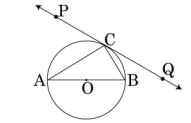
\includegraphics[width=5cm]{figs/1.png}
	\caption{}
\label{figure_1}
\end{figure} 
\item For what value of k will k+9, 2k-1 and 2k+7 are the consecutive terms of an A.P ?\\
\item A ladder, leaning against a wall, makes an angle of 60 \degree with the horizontal.If the foot of the ladder is 2.5 m away from the wall, find the length of the ladder.\\
\item A card is drawn at random from a well shuffled pack of 52 playing cards. Find the probability of getting neither a red card nor a queen.\\
\end{enumerate}

\section{\textbf{B}}
\textbf{Questions carry 2 marks each.}
\begin{enumerate}[label=\thesection.\arabic*.,ref=\thesection.\theenumi]
\item If -5 is a root of the quadratic equation $2x^2+px-15=0$ and the quadratic equation $p\brak{x^2+x}+k=0 $ has equal roots, find the value of k. \\
\item Solve for $x$ : $\sqrt{2x+9} + x = 13$ \\
\item Solve for $x$ : $\sqrt{6x+7}-\brak{2x-7}= 0$ \\
\item  Let P and Q be the points of trisection of the line segment joining the points A(2,-2) and B(-7, 4) such that P is nearer to A. Find the coordinates of P and Q.\\
\item  In Fig \ref{figure_2}, a quadrilateral ABCD is drawn to circumscribe a circle, with centre O, in such a way that the sides AB, BC, CD and DA touch the circle at the points P, Q, R and S respectively. Prove that $ AB + CD= BC + DA $.\\
	\begin{figure}[h!]
\centering
      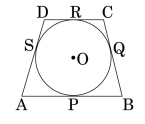
\includegraphics[width=5cm]{figs/2.png}
      \caption{}
      \label{figure_2}
\end{figure} 
\item  Prove that the points $\myvec{3,0}, \myvec{6, 4}$ and $\myvec{-1, 3}$ are the vertices of a right angled isosceles triangle.\\
\item  The 4th term of an A.P. is zero. Prove that the 25th term of the A.P. is three times its 11th term.\\
\item  In Fig \ref{figure_3}, from an external point P, two tangents PT and PS are drawn to a circle with centre O and radius r. If OP = 2r, show that $\angle OTS $ = $\angle OST $ = 30\degree.
\begin{figure}[h!]
\centering
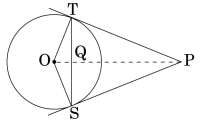
\includegraphics[width=5cm]{figs/3.png}
\caption{}
      \label{figure_3}
   \end{figure} 
   \end{enumerate}
\section{\textbf{C}}
\textbf{Questions carry 3 marks each.} \\
\begin{enumerate}[label=\thesection.\arabic*.,ref=\thesection.\theenumi]
\item  In fig \ref{figure_4}, $O$ is the centre of a circle such that diameter $AB = 13$ cm and $AC = 12$ cm. $BC$ is joined. Find the area of the shaded region. (Take $\pi = 3.14$)\\

	\begin{figure}[h!]
      \centering
      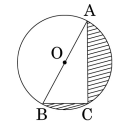
\includegraphics[width=5cm]{figs/4.png}
      \caption{}
      \label{figure_4}
\end{figure} 

\item  In \ref{figure_5}, a tent is in the shape of a cylinder surmounted by a conical top of same diameter. If the height and diameter of cylindrical part are 2.1 m and 3 m respectively and the slant height of conical part is 2.8 m, find the cost of canvas needed to make the tent if the canvas is available at the rate of Rs. 500/sq.metre. (Use $\pi$ = $\frac{22}{7}$)\\
	\begin{figure}[h!]
      \centering
      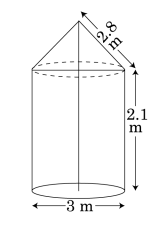
\includegraphics[width=5cm]{figs/5.png}
      \caption{}
      \label{figure_5}
\end{figure} 

\item  If the point $P\myvec{x, y}$ is equidistant from the points $A\myvec{a+b, b-a}$ and $B\myvec{a-b, a+b}$. Prove that bx=ay.\\
   
\item  In \ref{figure_6}, find the area of the shaded region, enclosed between two concentric circles of radii 7 cm and 14 cm where $\angle AOC$ = $40\degree$. (Use $\pi$ = $\frac{22}{7}$).
	\begin{figure}[h!]
      \centering
      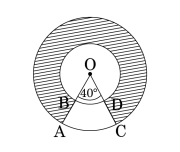
\includegraphics[width=5cm]{figs/6.png}
      \caption{}
      \label{figure_6}
\end{figure} 

\item  If the ratio of the sum of first n terms of two A.P's is (7n + 1) : (4n + 27), find the ratio of their m th terms.\\
\item There are 100 cards in a bag on which numbers from 1 to 100 are written. A card is taken out from the bag at random. Find the probability that the number on the selected card (i) is divisible by 9 and is a perfect square
(ii) is a prime number greater than 80.\\
\item Three consecutive natural numbers are such that the square of the middle number exceeds the difference of the squares of the other two by 60. Find the numbers.\\
\item The sums of first $n$ terms of three arithmetic progressions are $S_1, S_2$ and $S_3$ respectively. The first term of each A.P. is 1 and their common differences are 1, 2 and 3 respectively. Prove that $S_1+S_3=S_2$.\\
\item The digits of a positive number of three digits are in A.P. and their sum is 15.The number obtained by reversing the digits is 594 less than the original number. Find the number.\\
\item If the roots of the quadratic equation $\brak{a-b}x^2+\brak{b-c}x+\brak{c-a}=0$ are equal,prove that $2a=b+c$.\\
\item  Solve for $ x :  \frac{1}{(x-1)(x-2)} $ + $ \frac{1}{(x-2)(x-3)} $ = $ \frac{2}{3}$ , x $\neq$ 1,2,3   \\     
\item  A conical vessel, with base radius 5 cm and height 24 cm, is full of water. This water is emptied into a cylindrical vessel of base radius 10 cm. Find the height to which the water will rise in the cylindrical vessel. (Use $ \pi  = \frac{22}{7}$)\\

\item  A sphere of diameter 12cm, is dropped in a right circular cylindrical vessel, partly filled with water. If a sphere is completely submerged in water, the water level in the cylindrical vessel rises by $ 3 \frac{5}{9}$cm. Find the diameter of the cylindrical vessel.\\  

\item  A man standing on the deck of a ship, which is 10 m above water level, observes the angle of elevation of the top of a hill as $ 60\degree $ and the angle of depression of the base of hill as $ 30 \degree $. Find the distance of the hill from the ship and the height of the hill.\\
\item From a pack of 52 playing cards, Jacks, Queens and Kings of red colour are removed. From the remaining, a card is drawn at random. Find the probability that drawn card is :
(i) a black King (ii) a card of red colour (iii) a card of black colour\\
\item  Three different coins are tossed together. Find the probability of getting (i) exactly two heads (ii) at least two heads (iii) at least two tails.\\
\end{enumerate}

\section{\textbf{D}}  
\textbf{Questions carry 4 marks each.} \\
\begin{enumerate}[label=\thesection.\arabic*.,ref=\thesection.\theenumi]
\item  Due to heavy floods in a state, thousands were rendered homeless. 50 schools collectively offered to the state government to provide place and the canvas for 1500 tents to be fixed by the government and decided to share the whole expenditure equally. The lower part of each tent is cylindrical of base radius 2.8 m and height 3.5 m, with conical upper part of same base radius but of height 2.1 m. If the canvas used to make the tents costs \rupee~120 per sq.m, find the amount shared by each school to set up the tents. What value is generated by the above problem ? (Use $ \pi = \frac{22}{7} ) $\\
 
\item Prove that the lengths of the tangents drawn from an external point to a circle are equal.\\
\item Draw a circle of radius 4 cm. Draw two tangents to the circle inclined at an angle of $ 60 \degree $ to each other.\\
\item Draw a triangle with sides 5 cm, 6 cm and 7 cm. Then draw another triangle whose sides are $\frac{4}{5}$ of the corresponding sides of first triangle.\\
\item Draw an isosceles $\triangle ABC$ in which $BC=5.5 cm$ and altitude $AL=5.3 cm$. Then construct another triangle whose sides are $\frac{3}{4}$ of the corresponding sides of $\triangle ABC$.\\
\item Two pipes running together can fill a tank in $11\frac{1}{5}$ minutes. If one pipe takes 5 minutes more than the other to fill the tank separately, find the time in which each pipe would fill the tank separately.\\
\item In Fig \ref{figure_7} , two equal circles, with centres O and O', touch each other at X.OO' produced meets the circle with centre O' at A. AC is tangent to the circle with centre O, at the point C. O'D is perpendicular to AC. Find the value of $\frac{DO'}{CO}$.\\
	\begin{figure}[h!]
      \centering
      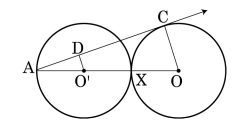
\includegraphics[width=5cm]{figs/7.png}
      \caption{}
      \label{figure_7}
   \end{figure} 
 
\item  Solve for $ x :  \frac{1}{x+1}  + \frac{2}{x+2}  = \frac{4}{x+4} , x \neq -1,-2,-4 .$ \\

\item The angle of elevation of the top $Q$ of a vertical tower $PQ$ from a point $X$ on the ground is $ 60\degree $. From a point $Y$, 40 m vertically above $X$, the angle of elevation of the top $Q$ of tower is $ 45 \degree $. Find the height of the tower PQ and the distance $PX$. ( Use $ \sqrt{3} = 1.73 $ ).\\
 
\item The houses in a row are numbered consecutively from 1 to 49. Show that there exists a value of $X$ such that sum of numbers of houses proceeding the house numbered $X$ is equal to sum of the numbers of houses following X.\\

\item A rectangular park is to be designed whose breadth is 3 m less than its length.Its area is to be 4 square metres more than the area of a park that has already been made in the shape of an isosceles triangle with its base as the breadth of the rectangular park and of altitude 12 m. Find the length and breadth of the rectangular park.\\

\item In fig \ref{figure_8}, the vertices of $\triangle ABC$ are $A\myvec{4, 6}, B\myvec{1, 5}$and $C\myvec{7, 2}$. A line-segment $DE$ is drawn to intersect the sides $AB$ and $AC$ at $D$ and $E$ respectively such that $\frac{AD}{AB}$ = $\frac{AE}{AC}$ = $\frac{1}{3}$ . Calculate the area of \( \Delta ADE \) and compare it with area of $ \triangle ABC$.\\
	\begin{figure}[h!]
      \centering
      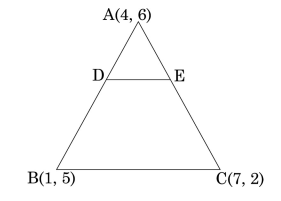
\includegraphics[width=5cm]{figs/8.png}
     \caption{}
      \label{figure_8}
\end{figure} 

\item A number $x$ is selected at random from the numbers 1, 2, 3 and 4. Another number $y$ is selected at random from the numbers 1, 4, 9 and 16. Find the probability that product of $x$ and $y$ is less than 16.\\

\item In Fig  \ref{figure_9} , is shown a sector $OAP$ of a circle with centre $O$, containing $\angle \theta$. $AB$ is perpendicular to the radius $OA$ and meets $OP$ produced at $B$. Prove that the perimeter of shaded region is $r$ $\left[\tan \theta + \sec \theta + \frac{\pi \theta}{180}-1 \right] $ \\

	\begin{figure}[h!]
      \centering
      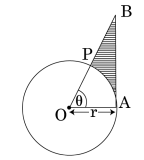
\includegraphics[width=5cm]{figs/9.png}
     \caption{}
     \label{figure_9}
\end{figure} 


\item A motor boat whose speed is 24 km/h in still water takes 1 hour more to go 32 km upstream than to return downstream to the same spot. Find the speed of the stream.\\
\end{enumerate}
\end{document}
